%%%%%%%%%%%%%%%%%%%%%%%%%%%%%%%%%%%%%%%%%%%%%%%%%%%%%%%%%%%%%%%%
% %
% Due Date %
% Andrew Gibson %
% ECE 351 lab, Section 53 %
% Lab 6 %
% Due 28 Feb 2023 %
% Step and Impulse Response of an RLC Bandpass Filter %
%https://github.com/gibs0630/ECE351\_Code %
%https://github.com/gibs0630/ECE351\_Reports %
% %
%%%%%%%%%%%%%%%%%%%%%%%%%%%%%%%%%%%%%%%%%%%%%%%%%%%%%%%%%%%%%%%%

\documentclass[12pt,a4paper]{article}
\usepackage[utf8]{inputenc}
\usepackage[greek,english]{babel}
\usepackage{alphabeta} 
\usepackage[pdftex]{graphicx}
\usepackage[top=1in, bottom=1in, left=1in, right=1in]{geometry}
\linespread{1.06}
\setlength{\parskip}{8pt plus2pt minus2pt}
\widowpenalty 10000
\clubpenalty 10000
\newcommand{\eat}[1]{}
\newcommand{\HRule}{\rule{\linewidth}{0.5mm}}
\usepackage[official]{eurosym}
\usepackage{enumitem}
\setlist{nolistsep,noitemsep}
\usepackage[hidelinks]{hyperref}
\usepackage{cite}
\usepackage{lipsum}

\newcommand{\Q}{\leavevmode\par\textbf {Q:}}
\newcommand{\A}{\par\textbf{A:} \normalfont}

\hypersetup{colorlinks=true, linkcolor=black, urlcolor=blue}

\begin{document}
%===========================================================
\begin{titlepage}
\begin{center}
% Top 
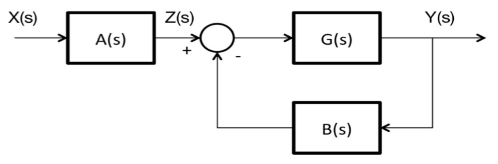
\includegraphics[width=0.55\textwidth]{titlepage_image.png}~\\[2cm]
% Title
\HRule \\[0.4cm]
{ \LARGE 
  \textbf{Project Report for ECE 351}\\[0.4cm]
  \emph{Lab 7: Block Diagrams and System Stability}\\[0.4cm]
}
\HRule \\[1.5cm]
% Author
{ \large
  Andrew Gibson \\[0.1cm]
 28 February 2023\\[0.1cm]
  \url{https://github.com/gibs0630/ECE351\_Code}\\[0.1cm]
  \url{https://github.com/gibs0630/ECE351\_Reports}\\[0.1cm]
  %#\texttt{user@cut.ac.cy}
}
\vfill
%\textsc{\Large Cyprus University of Technology}\\[0.4cm]\textsc{\large Department of Electrical Engineering,\\Computer Engineering \& Informatics}\\[0.4cm]
% Bottom
{\large }
 
\end{center}
\end{titlepage}
%\begin{abstract}
%\lipsum[1-2]
%\addtocontents{toc}{\protect\thispagestyle{empty}}
%\end{abstract}
\newpage
%===========================================================
\tableofcontents
\addtocontents{toc}{\protect\thispagestyle{empty}}
\newpage
\setcounter{page}{1}
%===========================================================
%===========================================================
\section{Introduction}\label{sec:intro}
With a block diagram of signal flow in the s-domain, it can be tedious to do algebraic calculations by hand.  Using python software, it can be trivial to conduct analysis  on various transfer functions that interact via the block diagram rules if they are composed of polynomials or polynomials divided by polynomials. 

\section{Equations}\label{sec:lit-rev}


equations from the lab
\[G(s) = \frac{s+9}{(s^2-6s-16)(s+4)}\]
\[A(s) = \frac{s+4}{(s^2+4s+3)(s+4)}\]
\[B(s) = s^2+26s+168\]

\section{Methodology}\label{sec:meth}
This lab had us find poles and zeroes of transfer functions in the s domain. Part one was an analysis of the open-loop transfer function, A(s) times G(s), while part 2 was an analysis of a closed-loop transfer function, where there is feedback from B(s). 

\section{Results}\label{sec:res}
\subsection*{Part 1}
task 1\\
\[G(s) = \frac {(s+9)}{(s^2-6s-16)(s+4)}\]
\[G(s) = \frac {A}{(s+4)} + \frac {B}{(s-8)} + \frac{C}{(s+2)}\]

\[A= \left . \frac {(s+9)}{(s-8)(s+2)} \right | _{n=-4} = \frac {((-4)+9)}{(((-4)-8)((-4)+2)} = \frac {1}{24}\]
\[B= \left . \frac {(s+9)}{(s+4)(s+2)} \right|_{n=8} = \frac {((8)+9)}{(((8)+4)((8)+2))} = \frac {17}{120}\]
\[C= \left . \frac {(s+9)}{(s+4)(s-8)} \right|_{n=-2} = \frac {((2)+9)}{(((2)+4)((2)-8))} = \frac {-11}{36}\]

\[G(s) = \frac {(1/24)}{(s+4)} + \frac {(17/120)}{(s-8)} + \frac {(-11/36)}{(s+2)}\]
poles are -4, 8, -2\\
zeroes are -9\\

\[A(s) = \frac {(s+4)}{(s^2+4s+3)}\]
\[A(s) = \frac {B}{(s+3)} + \frac {C}{(s+1)}\]

\[B=\left . \frac {(s+4)}{(s+1)} \right|_{n=-3} = \frac {((-3)+4)}{((-3)+1)} = \frac {1}{2}\]
\[C=\left . \frac {(s+4)}{(s+3)} \right|_{n=-1} = \frac {((-1)+4)}{((-1)+3)} = \frac {3}{2}\]

\[A(s) = \frac {(1/2)}{(s+3)} + \frac {(3/2)}{(s+1)}\]
poles are -1, -3\\
zeroes are -4 \\
\[B(s) = s^2+26s+168\]
\[B(s) = (s+12)(s+14)\]
there are no poles\\
zeroes are -12 and -14\\

task 2\\
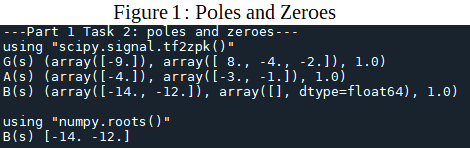
\includegraphics[width=0.55\textwidth]{Figure1.png}\\
The purpose producing Figure 1 was to show the output of the scipy.signal.tf2zpk function for finding the poles, roots, and gains. If the denominator is 1, then the numpy.roots function can be used instead to find the roots of a polynomial.


task 3\\
\[Y = G*A*X\]

\[Y(s) = \left (\frac {(s+9)}{(s+4)(s-8)(s+2)}\right)*\left( \frac{(s+4)}{(s+3)(s+1)}\right)*X(s)\]
\[Y(s) = \frac {(s+9)(s+4)}{(s+4)(s-8)(s+2)(s+3)(s+1)}*X(s)\]

\[Y(s) = \frac{(s+9)}{(s-8)(s+2)(s+3)(s+1)}*X(s)\]

task 4\\
The open-loop response is not stable because of the $(s-8)$ term in the denominator. when converting that term to time domain, there will be an $e^{-(-8)t}$, and $e^{8t}$ does not converge to a finite number as t approaches infinity

task 5\\
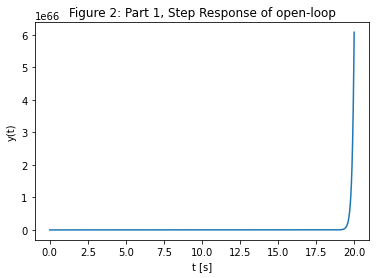
\includegraphics[width=0.55\textwidth]{Figure2.png}\\
The purpose producing Figure 2 was to show that the transfer function of the open-loop is unstable. 

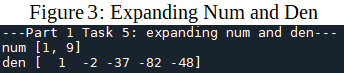
\includegraphics[width=0.55\textwidth]{Figure3.png}\\
The purpose producing Figure 1 was to show the the zeroes and holes. notice that one of the terms when they are multiplied together.

\[Y(s) = \frac {s+9} {s^4-2s^3-37s^2-82s-48}\]

task 6\\
The result of task 5 corresponds to the results of task4 as the graph grows exponentially which as t becomes large.



\subsection*{Part 2}
task 1\\
\[Y = G*E\]
\[E=A*X-B*Y\]

\[A*X-B*Y = \frac Y G\]
\[A*X = \frac Y G +B*Y\]
\[G*A*X = Y+G*B*Y\]
\[G*A*X = Y(1+G*B)\]
\[Y = \frac {G*A*X} {1+G*B }\]
\[H = \frac{G*A}{1+G*B}\]


\[H = \frac {\frac{numG}{denG}* \frac{numA}{denA}}{1+\frac {numG}{denG}*\frac{numB}{denB}}\]
\[H = \frac {\frac{numG*numA}{denG*denA}}{(1+\frac{numG*numB}{denB*denG}}\]
\[H = \frac {\frac{(numG*numA)(denB*denG)}{denG*denA}}{denB*denG+numG*numB}\]
\[H = \frac {(numG*numA)(denB*denG)}{(denB*denG)(denG*denA)+(numG*numB)(denG*denA)}\]
\[H = \frac {numG*numA*denB*denG}{denB*denG*denG*denA+numG*numB*denG*denA}\]
\[H = \frac {numG*numA*denB}{denB*denG*denA + numG*numB*denA}\]


task 2\\
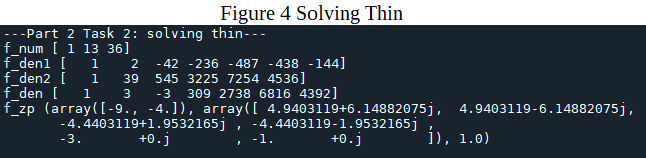
\includegraphics[width=0.55\textwidth]{Figure4.png}\\
The purpose producing Figure 1 was to show convolving in s domain to find the terms and roots

\begin{equation}
\tiny
\frac{(s+9)(s+4)} {(s-(4.9403+6.1488j)(s-(4.9403-6.1488j))(s-(-4.4403+1.9532j))(s-(-4.4403-1.9532j))(s+3)(s+1) }
\end{equation}

task 3\\
because there are complex roots, there is no convergence to a single value.however, those roots could cause the system explode.

Take the inverse Laplace of the term $\frac 1 {s+a+bj}$
\[e^{-(a+bj)t}\]
\[e^{-at}*e^{-bjt}\]
\[e^{-at}*(e^{jt})^{-b}\]
\[e^{-at}*(cos(t)+j sin(t))^{-b}\]

Therefore as long as the real components of the zeros are all negative, then  there would be stability. 
This system is still unstable even with the feedback, and it will oscillate in which direction it is unstable


task 4\\
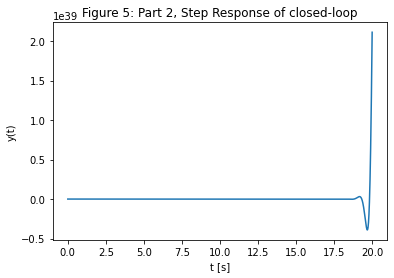
\includegraphics[width=0.55\textwidth]{Figure5.png}\\
The purpose producing Figure 4 was to show that the transfer function of the closed-loop is unstable.  Even though it oscillates, the magnitude keeps growing.\\


task 5\\
The result of task 4 corresponds to the results of task3 as the graph grows exponentially larger (albeit periodically) as t becomes large.



\section{Questions}\label{sec:res}

\Q 1. In Part 1 Task 5, why does convolving the factored terms using scipy.signal.convolve() result in the expanded form of the numerator and denominator? Would this work with your user-defined convolution function from Lab 3? Why or why not? 
\A 1. the scipy.signal.convolve() function works with the coefficients of a numerator and denomenator in the s domian.  It would not work in the time domain.  You can do a discrete convolution in the time domain with numpy.convolve. The user defined function in Lab 3 is also a descrete convolution in the time domain.  Scipy.signal.convolve and the user defined function in lab 3 are not compatible

\Q 2. Discuss the difference between the open- and closed-loop systems from Part 1 and Part 2. How does stability differ for each case, and why?
\A 2. The open end system  has a signal going one way and no feed back, however the output is unstable, the closed system  has a feedback loop that is also unstable but does not converge as t approaches infinity.

\Q 3. What is the difference between scipy.signal.residue() used in Lab 6 and scipy.signal.tf2zpk() used in this lab?
\A 3. the function scipy.signal.residue() numerator and denominator coefficients in the s domain and returns the partial-fraction expansion with the residue corresponding to the poles, the poles, and any standalone coefficients. the function scipy.signal.tf2zpk also takes numerator and denominator coefficients but returns the values of s to cause it to equal zero (zeroes), the values of s where it is undefined (poles), and the gain.

\Q 4. Is it possible for an open-loop system to be stable? What about for a closed-loop system to be unstable? Explain how or how not for each.
\A 4. it is possible for an open-loop to system to be stable as it would need a term that had a positive pole. Same goes for closed-loop systems.

\Q 5. Leave any feedback on the clarity/usefulness of the purpose, deliverable, and expectations for this lab.
\A 5. Some time was wasted calculating y(t) because of a type in the procedure.
also it was unclear if we were suppose to work only in the s domain.
 it is also unclear how to add the coefficients together two numpy.arrays,which is what scipy.signal uses that are of different lengths. The feedback system had such a case where we needed to do that to get the terms.



%\lipsum[7-8]\cite{knuthwebsite}
%===========================================================
%===========================================================
\bibliographystyle{ieeetr}
\bibliography{refs}
\end{document} 
Annotations











